% !TEX program = pdflatex
% !TEX encoding = UTF-8
%
% IEEE Conference Paper Template
% Version: 2.0
% Last Updated: 2026/01/26
% GitHub: https://github.com/EmpyreanHYR/Self-made-LaTeX-Template-for-IEEE-Conferences
%

\documentclass[conference]{IEEEtran}

\IEEEoverridecommandlockouts
% The preceding line is only needed to identify funding in the first footnote. If that is unneeded, please comment it out.

% ==================== 引用和参考文献 ====================
\usepackage[sort&compress,numbers]{natbib}  % BibTeX方式（需要.bib文件）
% \usepackage{cite}  % 手动\bibitem方式
% cite包默认自动排序和压缩引用，如 [2, 3] 和 [4-7]
% 自定义cite格式以匹配IEEE样式
\renewcommand{\citepunct}{, }           % 引用之间用逗号和空格分隔
\renewcommand{\citedash}{--}            % 连续引用用双连字符

% ==================== 数学相关宏包 ====================
\usepackage{amsmath,amssymb,amsfonts}  % AMS数学宏包套件
\usepackage{mathtools}                  % 数学工具增强
\usepackage{bm}                         % 粗体数学符号
% \usepackage{mathrsfs}                 % 花体字母（可选）

% ==================== 算法相关宏包 ====================
\usepackage{algorithmic}                % 传统算法环境
\usepackage{algorithm}                  % 算法浮动体环境
% \usepackage[ruled,vlined]{algorithm2e} % 现代算法宏包（与algorithmic二选一）

% ==================== 图形和颜色 ====================
\usepackage{graphicx}                   % 图形插入
\usepackage{xcolor}                     % 颜色支持
\usepackage{float}                      % 浮动体控制
\usepackage{subfig}                     % 子图支持
% \usepackage{subcaption}               % 子图替代方案（与subfig二选一）
\usepackage{dblfloatfix}                % 修复双栏浮动体问题
\setcounter{dbltopnumber}{2}            % 允许同页顶部放置两张跨栏表
\renewcommand{\dbltopfraction}{0.95}    % 跨栏表可占页面顶部较大区域
\renewcommand{\textfraction}{0.05}      % 避免宽表被推迟到独立页面
\renewcommand{\figurename}{Figure}      % 图标题英文化

% ==================== 表格相关宏包 ====================
\usepackage{booktabs}                   % 专业三线表
\usepackage{tabularx}                   % 可伸缩表格
\usepackage{multirow}                   % 跨行单元格
\usepackage{makecell}                   % 单元格内换行和格式化
\usepackage{array}                      % 表格列格式增强
% \usepackage{longtable}                % 跨页长表格

% ==================== 文本和字体 ====================
\usepackage{textcomp}                   % 文本符号补充
\usepackage{soul}                       % 文本高亮和下划线
\usepackage[normalem]{ulem}             % 各种下划线样式（normalem保护\emph）
% \usepackage{xspace}                   % 智能空格处理

% ==================== 代码展示 ====================
\usepackage{listings}                   % 代码高亮显示
\lstset{
    basicstyle=\ttfamily\small,
    breaklines=true,
    frame=single,
    numbers=left,
    numberstyle=\tiny,
    keywordstyle=\color{blue},
    commentstyle=\color{green!50!black},
    stringstyle=\color{red}
}

% ==================== 链接和引用 ====================
\usepackage{url}                        % URL格式化
\usepackage{hyperref}                   % 超链接支持（必须在大多数包之后）
\hypersetup{
    colorlinks=true,        % 启用颜色链接
    allcolors=black,        % 所有链接颜色设为黑色
    pdfstartview=Fit,       % PDF打开时适配页面
    breaklinks=true,        % 允许链接换行
    pdftitle={Privacy-Preserving Edge-Cloud Fall Detection with Quality-Aware Bidirectional Temporal Modeling},
    pdfauthor={Course Project Team},
    pdfsubject={IoT Course Project Report},
    pdfkeywords={fall detection, skeleton sequence, temporal convolution, transformer, Mamba, missing observations}
}
\usepackage{cleveref}                   % 智能交叉引用（必须在hyperref之后）

% cleveref 配置 - IEEE会议论文格式
\crefname{figure}{Fig.}{Figs.}          % 图的引用格式
\Crefname{figure}{Figure}{Figures}      % 句首图的引用格式
\crefname{table}{Table}{Tables}         % 表的引用格式
\Crefname{table}{Table}{Tables}         % 句首表的引用格式
\crefname{equation}{Eq.}{Eqs.}          % 公式的引用格式
\Crefname{equation}{Equation}{Equations}% 句首公式的引用格式
\crefname{section}{Sec.}{Secs.}         % 节的引用格式
\Crefname{section}{Section}{Sections}   % 句首节的引用格式
\crefname{subsection}{Sec.}{Secs.}      % 子节的引用格式
\Crefname{subsection}{Section}{Sections}% 句首子节的引用格式
\crefname{algorithm}{Alg.}{Algs.}       % 算法的引用格式
\Crefname{algorithm}{Algorithm}{Algorithms}% 句首算法的引用格式
\crefname{listing}{Listing}{Listings}   % 代码清单的引用格式
\Crefname{listing}{Listing}{Listings}   % 句首代码清单的引用格式
\crefname{appendix}{Appendix}{Appendices}% 附录的引用格式
\Crefname{appendix}{Appendix}{Appendices}% 句首附录的引用格式

% cleveref 多引用格式配置
\newcommand{\crefrangeconjunction}{--}  % 范围连接符：Fig. 1--3
\newcommand{\crefpairconjunction}{ and }% 两个引用连接符：Fig. 1 and 2
\newcommand{\crefmiddleconjunction}{, } % 多个引用中间连接符：Fig. 1, 2, and 3
\newcommand{\creflastconjunction}{, and }% 多个引用最后连接符

% ==================== 其他实用工具 ====================
\usepackage{calc}                       % 计算功能
\usepackage{orcidlink}                  % ORCID链接
\usepackage{enumitem}                   % 列表环境定制
% \usepackage{siunitx}                  % 国际单位制符号
% \usepackage{tikz}                     % 绘图宏包

% ==================== 自定义命令 ====================
% BibTeX标志
\def\BibTeX{{\rm B\kern-.05em{\sc i\kern-.025em b}\kern-.08em
    T\kern-.1667em\lower.7ex\hbox{E}\kern-.125emX}}

% 作者换行命令
\makeatletter
\newcommand{\linebreakand}{%
  \end{@IEEEauthorhalign}
  \hfill\mbox{}\par
  \mbox{}\hfill\begin{@IEEEauthorhalign}
}
\makeatother

% ========== 常用自定义命令示例 ==========
% 取消下面的注释以启用这些命令

% 缩写命令
% \newcommand{\eg}{e.g.,\xspace}
% \newcommand{\ie}{i.e.,\xspace}
% \newcommand{\etc}{etc.\xspace}
% \newcommand{\etal}{et al.\xspace}

% 数学命令
% \newcommand{\R}{\mathbb{R}}          % 实数集
% \newcommand{\C}{\mathbb{C}}          % 复数集
% \newcommand{\N}{\mathbb{N}}          % 自然数集
% \newcommand{\norm}[1]{\left\|#1\right\|}  % 范数
% \newcommand{\abs}[1]{\left|#1\right|}     % 绝对值

% 文本强调
% \newcommand{\important}[1]{\textbf{#1}}  % 重要内容
% \newcommand{\term}[1]{\textit{#1}}       % 术语

\begin{document}

\title{Privacy-Preserving Edge--Cloud Fall Detection\\
with Quality-Aware Bidirectional Temporal Modeling}

\author{
\IEEEauthorblockN{Jiahao Zhao, Chengyi Xu, Yaorong Huang, Zhonglin Chang, and Jiayun Song}
\IEEEauthorblockA{Internet of Things Essentials, Faculty of Applied Sciences\\
Macao Polytechnic University, Macao SAR, China}
}




\maketitle

\begin{abstract}
Incomplete pose observations complicate camera-based fall detection, particularly when a short fall transition must be distinguished from daily activities. We propose MaskedBiMamba, a skeleton sequence classifier that combines bidirectional state-space modeling, temporal self-attention, frame masking, and aggregation guided by pose confidence. The model is integrated into an edge-cloud prototype with local Raspberry Pi pose extraction and classification, Hailo acceleration, persistent alerts, and a monitoring dashboard. Pending records are retained locally for cloud synchronization. We compare five temporal models over four subject-disjoint folds and three random seeds on CAUCAFall and GMDCSA-24. The Transformer encoder achieves the highest window F1 ($0.6581\pm0.0766$), while MaskedBiMamba achieves the highest window precision ($0.6048\pm0.0856$) and the lowest false-alarm rate ($198.5\pm40.8$ per evaluated video hour). Under 30\% random frame loss, MaskedBiMamba retains window F1 $0.6276\pm0.0507$, compared with $0.4361\pm0.0669$ for TCNTE; this robustness advantage also appears on external Le2i data. Ablations support bidirectional processing and temporal attention, while masking and quality pooling show trade-offs on clean inputs. The results favor MaskedBiMamba for tolerance to missing frames and precision, with spatial keypoint loss the main remaining error source.
\end{abstract}

\begin{IEEEkeywords}
fall detection, skeleton sequence, edge-cloud system, temporal attention, Mamba.
\end{IEEEkeywords}


\section{Introduction}

Falls can resemble sitting, kneeling, or lying down in a single frame. Their distinction depends on the descent and the posture that follows. Camera-based monitoring captures this motion without a wearable device, but furniture, lighting changes, and tracking failures can interrupt observations. Skeleton sequences describe body movement compactly while reducing the visual detail passed to the classifier. Their usefulness depends on temporal modeling and the reliability of estimated joints across successive video frames.

The intended setting is an indoor assisted-living space, where caregivers review suspected falls and acknowledge events through a monitoring interface. The design objectives are to process video near the camera, continue detection during network outages, and preserve event times when records reach the cloud after reconnection.

Recent work combines temporal operators for skeleton-based fall detection. Yu et al.~\cite{yu2025tcnte} proposed TCNTE, which couples dilated temporal convolutions with a Transformer encoder and uses weighted focal loss to address class imbalance. Their implementation integrates pose estimation and tracking on a Jetson edge device. Kim et al.~\cite{kim2025yosap} developed YOSAP-LSTM for construction scenes with occlusion. It combines person detection and tracking with AlphaPose and a one-dimensional CNN-LSTM classifier, with evaluation on an embedded platform. Both studies connect motion classification with the cost and observation errors of pose extraction.

Zhang et al.~\cite{zhang2025fallmamba} introduced Fall-Mamba, which uses cross-attention to fuse video and audio features, together with multihead temporal attention and frame masking. Its masked sequence modeling motivates studying temporal interruptions in pose sequences. Chun et al.~\cite{chun2025stonegat} proposed StoneGAT, a graph attention model for individual poses that uses bone-related edge attributes, including confidence information. Its PointOut strategy drops node features during training to study resilience to missing joints. Frame masking removes observations at selected times, whereas node removal reduces the body geometry available within an observation. These distinct losses motivate separate evaluation of temporal and spatial disruption.

We propose MaskedBiMamba to combine bidirectional state-space modeling with explicit pose-quality information. Forward and backward Mamba branches~\cite{gu2023mamba} relate each posture to surrounding motion within a buffered window; temporal attention connects observations, and a learned quality gate aggregates frame features. Training-time masking exposes the classifier to interrupted sequences. This design is evaluated against convolutional, attention-based, and unidirectional state-space alternatives. Component ablations examine attention, bidirectionality, masking, and quality pooling, while controlled perturbations separate frame loss, joint loss, and confidence noise. Window, video, and event measures describe classification and the false alarms produced by temporal aggregation. The system contribution embeds this classifier in a pose-based edge-cloud prototype, pairing on-device pose extraction with Hailo acceleration and an authenticated monitoring interface. Together, the architecture, experimental analysis, and operational alert workflow examine how a compact fall detector behaves under incomplete observations and changes in recording conditions.


\section{System design}
\label{sec:system}

FallGuard performs pose extraction and temporal classification on the Raspberry Pi. The Hailo accelerator runs the pose network, while the Pi CPU evaluates a one-second skeleton window with MaskedBiMamba. The local alert state and prediction records remain available during network outages. When connectivity returns, a synchronization service transfers pending records to the cloud for event history and dashboard updates. Figure~\ref{fig:edge_flow} shows this data flow.

\begin{figure*}[tp]
\centering
\begin{tikzpicture}[font=\small,box/.style={draw,rounded corners=2pt,align=center,minimum height=0.85cm,text width=2.25cm,fill=blue!4},arr/.style={-{Latex[length=2mm]},thick}]
\node[box] (camera) {Camera or local video};
\node[box,right=0.35cm of camera] (pose) {YOLOv8 pose\\Hailo / CPU};
\node[box,right=0.35cm of pose] (model) {1-s pose window\\MaskedBiMamba};
\node[box,right=0.35cm of model] (queue) {Local alert state\\SQLite records};
\draw[arr] (camera)--(pose);\draw[arr] (pose)--(model);\draw[arr] (model)--(queue);
\node[box,below=1.2cm of queue,fill=orange!6] (cloud) {Cloud event store\\and dashboard};
\draw[arr] ([xshift=-.35cm]queue.south)--node[left,font=\footnotesize,align=right]{Pending records\\on reconnection}([xshift=-.35cm]cloud.north);
\draw[arr] ([xshift=.35cm]cloud.north)--node[right,font=\footnotesize]{Acknowledgement}([xshift=.35cm]queue.south);
\begin{scope}[on background layer]
\node[draw,dashed,rounded corners,fit=(camera)(pose)(model)(queue),inner sep=8pt,label=above:{Raspberry Pi: inference continues without a network}] {};
\end{scope}
\end{tikzpicture}
\caption{Local inference and deferred cloud synchronization. CPU pose estimation provides a fallback when the Hailo backend is unavailable. Cloud acknowledgement follows durable storage, allowing safe retries after an interrupted transfer.}
\label{fig:edge_flow}
\end{figure*}

Routine synchronization transfers pose features and classification records. An authenticated preview can relay annotated images for monitoring; preview frames are held temporarily and kept separate from the event archive.

\subsection{Alert-state transitions}

The edge node converts a sequence of fall probabilities into \textsc{Normal}, \textsc{Suspected}, \textsc{Confirmed}, and \textsc{Cleared} states. Let $p_k$ be the probability of the $k$th locally classified window. The high- and low-probability counters are
\begin{equation}
\begin{aligned}
 c_k^+ &= \mathbf{1}[p_k\geq0.65](c_{k-1}^++1),\\
 c_k^- &= \mathbf{1}[p_k\leq0.35](c_{k-1}^-+1).
\end{aligned}
\label{eq:alert_counters}
\end{equation}
A high observation opens a suspected event. Confirmation requires $c_k^+\geq2$ and $p_k\geq0.82$; $c_k^-\geq2$ clears an active event. Requiring consecutive high-probability observations prevents an isolated spike from confirming an event. Acknowledgement and user notes are stored with the event, separately from the prediction sequence.


\section{Temporal Detection Method}

\subsection{Data and Pose Caching}

The experiments use Le2i and CAUCAFall, summarized in Table~\ref{tab:datasets}. Le2i was introduced as a realistic single-camera fall-detection benchmark with changes in scene, viewpoint, clothing, illumination, shadow, and occlusion~\cite{charfi2012le2i}. The released annotated subset used by TCNTE is commonly reported as 191 videos (48 ADL and 143 fall videos), recorded at $320\times240$ pixels and 25 fps~\cite{yu2025tcnte}. The local archive contained 190 decodable videos, which were distributed over six recording-scene groups. Because reliable participant identifiers were absent from this copy, scenes rather than nominal subjects were used for leakage control.

CAUCAFall was collected in an intentionally uncontrolled home environment. Ten participants each performed five fall types---forward, backward, left, right, and from sitting---and five ADLs---walking, hopping, picking up an object, sitting, and kneeling~\cite{guerrero2022caucafall}. Its 100 videos were recorded at $1080\times960$ pixels and 23 fps under natural, artificial, and night lighting, with variation in clothing, occlusion, background motion, fall angle, and camera distance. Subject folders are retained, enabling subject-disjoint folds. CAUCAFall additionally provides frame-level fall/no-fall and person-region labels, although this work uses the videos and temporal labels rather than training a frame detector.

\begin{table*}[!t]
    \centering
    \small
    \caption{Datasets used in this study. ``Reported'' describes the source publication or commonly used released subset; ``used'' is the number successfully processed by our pipeline.}
    \label{tab:datasets}
    \begin{tabularx}{\textwidth}{>{\raggedright\arraybackslash}p{1.8cm}>{\raggedright\arraybackslash}p{2.6cm}>{\raggedright\arraybackslash}p{3.1cm}>{\raggedright\arraybackslash}p{2.8cm}>{\raggedright\arraybackslash}p{2.8cm}X}
        \toprule
        Dataset & Videos & Subjects/groups & ADL/fall types & Resolution and rate & Role in this study \\
        \midrule
        Le2i & 191 reported (48/143 ADL/fall); 190 used & 9 subjects reported; 6 scene groups used & 6 ADL / 3 fall types & $320\times240$, 25 fps & TCNTE reproduction and primary comparison \\
        CAUCAFall & 100 reported and used (50/50 ADL/fall) & 10 subject groups & 5 ADL / 5 fall types & $1080\times960$, 23 fps & Primary comparison only \\
        \bottomrule
    \end{tabularx}
\end{table*}

The resulting 290 videos contain 967 Le2i and 258 CAUCAFall annotation segments. The positive label \emph{fall} denotes the dynamic transition; post-fall \emph{fallen} intervals are not merged into the positive class. A pretrained YOLOv8s-pose model with BoT-SORT tracking extracts one primary person track per video. Each cache stores timestamps, 17 COCO keypoints and their confidence values, a normalized person box, detector confidence, and the track identifier.

Only the 12 non-face body joints are used by the temporal classifiers. For each frame, coordinates are independently min--max normalized over the retained joints. The TCNTE reproduction uses $(x,y)$ and therefore has 24 input features per frame. The primary protocol additionally uses pose confidence, yielding 36 features. Three observation-quality features are retained at each time step: mean keypoint confidence, the proportion of joints with confidence at least 0.2, and person-box confidence.

\subsection{Window Construction and Data Splits}

Each window spans 1.0~s, consecutive windows begin 0.2~s apart, and every window is linearly resampled to 30 time steps. A window is positive when at least 50\% of its duration overlaps a fall segment. Windows with nonzero but sub-threshold overlap are discarded to avoid ambiguous transition labels. For videos containing a fall, windows beginning after the last annotated fall transition are excluded from the reproduction protocol.

Two protocols are reported separately. The paper-aligned TCNTE reproduction uses Le2i with three video-grouped folds and reserves 15\% of the non-test videos for validation. It contains 12,650 windows in total: 1,338 positive and 11,312 negative windows. The primary protocol combines Le2i and CAUCAFall in four group-disjoint folds. CAUCAFall is grouped by its 10 subject identifiers; because reliable Le2i subject identifiers are unavailable, its six recording scenes are used as groups. Dataset names prefix every group identifier to prevent accidental collisions.

\subsection{Compared Temporal Models}

All models receive the same window manifest within a protocol. The TCN contains three residual temporal blocks with channels $[8,16,32]$, kernel size 5, dilations $1,2,4$, and dropout 0.2. The Transformer encoder (TE) linearly projects each frame to 32 dimensions, adds learned positional encoding, and applies one four-head encoder layer with a feed-forward width of 32. TCNTE passes the TCN sequence to the same encoder before temporal mean pooling.

The state-space baseline, UniMamba, projects each frame to 64 dimensions and uses two unidirectional Mamba layers with state size 16, convolution width 4, and expansion factor 2. The proposed MaskedBiMamba first masks 15\% of frames during training and applies temporal self-attention. Independent forward and reverse Mamba stacks encode the sequence, after which their outputs are concatenated and linearly fused. A learned scalar gate $a_t$ is computed from the three-dimensional quality vector $\mathbf q_t$ and used for temporal aggregation:
\begin{equation}
    \mathbf z = \frac{\sum_{t=1}^{T} a_t\mathbf h_t}{\sum_{t=1}^{T}a_t},
    \qquad
    a_t = \sigma\!\left(g(\mathbf q_t)\right).
\end{equation}
The pooled representation $\mathbf z$ is classified as fall or non-fall. This skeleton model is inspired by masked Mamba modeling but is not presented as an exact reproduction of the multimodal Fall-Mamba architecture.

\subsection{Optimization and Model Selection}

All models are trained for 100 epochs using Adam with learning rate $10^{-4}$, batch size 64, and weighted focal loss with $\gamma=3$. The TCNTE reproduction uses class weights $[1,30]$; the primary protocol estimates class weights from the training partition only. The checkpoint with the highest validation F1 is used for test evaluation. The reproduction uses seed 42; the primary comparison uses seeds 42, 3407, and 2026. CUDA mixed precision and deterministic seeds are enabled, while nondeterministic fused attention kernels are disabled.


\section{System Implementation}

\subsection{Edge Pose Node and Transport}

The edge implementation targets a Raspberry Pi~5, USB camera, and YOLO26n-pose model~\cite{jocher2026yolo26}. The sender selects the highest-confidence person, normalizes 17 COCO keypoints, computes confidence summaries, and publishes at most five pose packets per second. Old packets are dropped on congestion. An optional annotated preview is relayed in memory for authenticated viewing and is separate from the inference packet.

The available AI HAT+~2 contains a Hailo-10H accelerator, but the recorded Hailo pose trial returned invalid landmark coordinates from the installed postprocessor. The software YOLO26n-pose sender is therefore the documented usable path. Accelerator speed is not inferred from this incomplete integration. The private Tailscale relay authenticates packets; the cloud puller rejects stale sequence numbers and sends fresh observations to a loopback backend. Separate credentials protect the two hops, and the public HTTPS gateway blocks pose-ingestion routes.

\subsection{Cloud Service and Operating Interface}

Deployment notes describe a Python~3.11 backend on an OpenCloudOS~9 cloud VM, with SQLite event storage and an authenticated Nginx HTTPS gateway. Server-Sent Events (SSE) update the dashboard. Both Pi COCO packets and browser landmarks can enter the selected temporal-model adapter. When its runtime or inference is unavailable, the Pi path falls back to an explicitly labeled geometry baseline. Model selection and initialization status must therefore be checked before interpreting a score.

The live model catalog references September~16 course-trained checkpoints, including MaskedBiMamba; these belong to the earlier Le2i--CAUCAFall experiment. They are not the September~18 subject-disjoint primary checkpoints evaluated in Section~\ref{sec:experiments}. The browser path uses MediaPipe landmarks and the Pi path uses YOLO26n-pose; the offline experiments use YOLOv8s-pose caches. The live adapter takes the latest 30 received frames without timestamp resampling. At the Pi limit of 5~Hz, their first-to-last span is at least 5.8~s, whereas training resamples a 1~s window. Extractor and temporal-scale differences require validation before transferring offline results.

Figure~\ref{fig:dashboard} shows the actual operating interface captured from an isolated local backend during this review. The operator selects a model, checks readiness, selects a camera source, and inspects the preview, pose panel, probability, and alert state. Alert history supports acknowledgement with notes, and Pi controls expose camera start/stop. In the captured session, the Pi relay was not configured and the model runtime was unavailable; no live prediction is claimed. A separate, explicitly labeled synthetic replay exercised event creation, SSE delivery, SQLite persistence, and acknowledgement. It validates application behavior, not fall-recognition accuracy or current remote-cloud availability.

\begin{figure*}[tp]
    \centering
    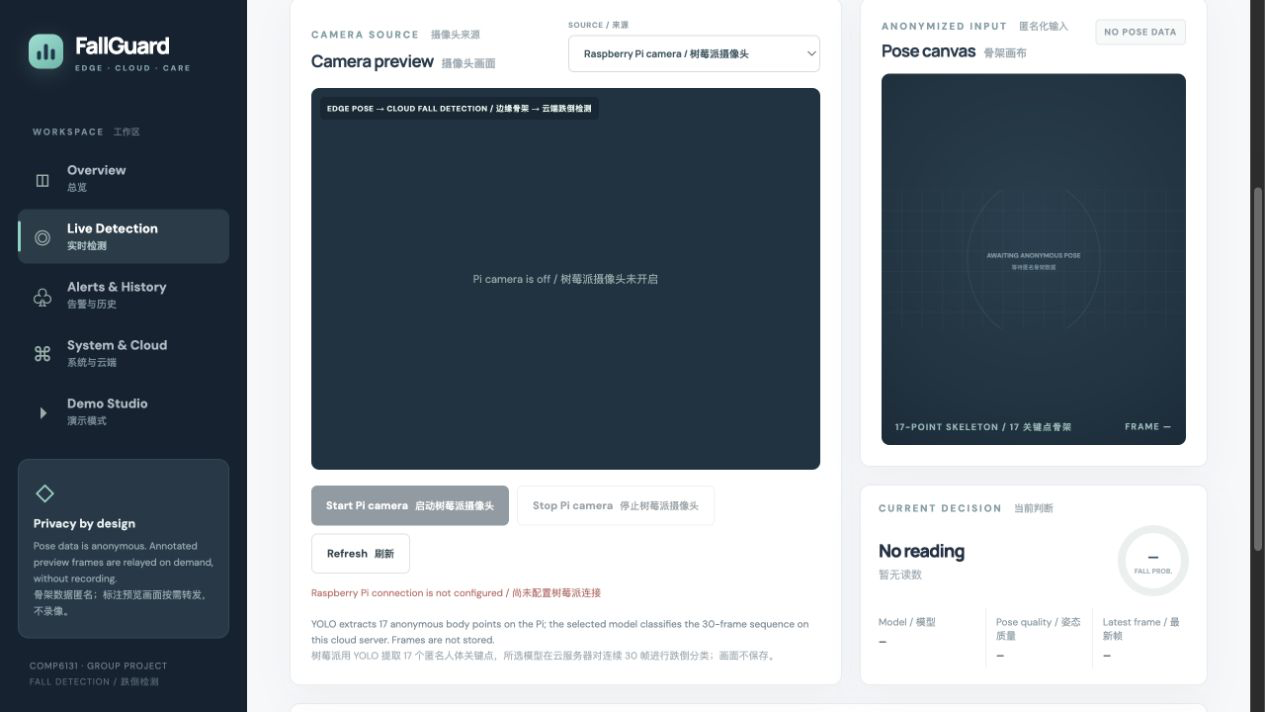
\includegraphics[width=0.96\textwidth,height=0.38\textheight,keepaspectratio]{figs/detection_system_ui_reviewed.png}
    \caption{Actual FallGuard operation interface from a local review session (September~19, 2026). Camera selection and controls, pose display, and current decision are visible. The camera and pose panels are idle: this local session had neither a configured Pi relay nor an available model runtime. This screenshot is interface evidence, not a cloud deployment benchmark.}
    \label{fig:dashboard}
\end{figure*}

\subsection{Reused Components and Project Additions}

The TCNTE paper and repository provide the baseline architecture~\cite{yu2025tcnte,tcnteCode}. The project reimplements its training pipeline with raw logits, a held-out validation split, and explicit configuration; it uses the paper's kernel size~5 rather than the released code's size~3. Ultralytics provides pretrained pose estimation~\cite{ultralyticsPose}, and \texttt{mamba-ssm} provides Mamba layers~\cite{mambaCode}. The ONNX wrapper uses mean joint confidence in place of detector-box confidence for its third quality feature. The project adds dataset adapters, frozen window protocols, confidence features, bidirectional fusion, quality pooling, retrained ablations, robustness evaluation, edge transport, the alert state machine, storage, and the dashboard. MaskedBiMamba is inspired by Fall-Mamba and is not its multimodal reproduction.

The project workspace contains \path{code/src/fallbench/models.py}, \path{engine.py}, frozen YAML configurations, and training/evaluation entry points. \path{webui/server.py}, \path{cloud_model.py}, and the edge/cloud subdirectories implement the demonstration. Dependency files and basic commands are in \path{code/README.md}, \path{webui/README.md}, and the reviewed report README. Per-run configurations, predictions, and metrics provide experiment provenance; the missing raw caches and original fold manifests must be restored for a full training replay.


\section{Experiments and Results}
\label{sec:experiments}

\subsection{Experimental Setting}

The positive class is \emph{fall}. Window-level reporting includes accuracy, precision, recall, F1, and AUROC at a fixed threshold of 0.5. A video is predicted as positive when any window reaches this threshold. Event recall measures the fraction of annotated fall intervals overlapped by at least one contiguous predicted interval, while false alarms per hour quantify erroneous alarms over negative video time. Tables~\ref{tab:environment} and~\ref{tab:configuration} summarize the execution environment and evaluation protocols. Each model in the primary comparison is evaluated over four folds and three random seeds.

\begin{table}[t]
    \centering
    \small
    \caption{Experimental execution environment.}
    \label{tab:environment}
    \begin{tabular}{ll}
        \toprule
        Item & Environment \\
        \midrule
        Operating system & Ubuntu 22.04, Linux 5.15 \\
        GPU & NVIDIA GeForce RTX 3090 \\
        Python & 3.10.8 \\
        PyTorch & 2.1.2+cu121 \\
        CUDA runtime & 12.1 \\
        Precision & Automatic mixed precision \\
        Reproducibility & Fixed seeds; deterministic mode \\
        \bottomrule
    \end{tabular}
\end{table}

\begin{table*}[!t]
    \centering
    \small
    \caption{Training and evaluation configurations.}
    \label{tab:configuration}
    \begin{tabular}{lll}
        \toprule
        Item & TCNTE reproduction & Primary comparison \\
        \midrule
        Dataset & Le2i & Le2i + CAUCAFall \\
        Input features & 12 joints $\times(x,y)$; 24 dimensions & 12 joints $\times(x,y,c)$; 36 dimensions \\
        Window / stride / resampling & 1.0 s / 0.2 s / 30 steps & 1.0 s / 0.2 s / 30 steps \\
        Split and validation & 3 video-grouped folds; 15\% validation & 4 group-disjoint folds; 20\% validation \\
        Random seeds & 42 & 42, 3407, 2026 \\
        Epochs / batch size & 100 / 64 & 100 / 64 \\
        Optimizer / learning rate & Adam / $10^{-4}$ & Adam / $10^{-4}$ \\
        Objective & Weighted focal loss, $\gamma=3$, weights $[1,30]$ & Weighted focal loss, $\gamma=3$, training-fold weights \\
        Checkpoint rule & Maximum validation F1 & Maximum validation F1 \\
        Test threshold & 0.5 & 0.5 \\
        \bottomrule
    \end{tabular}
\end{table*}

\subsection{TCNTE Reproduction}

Table~\ref{tab:tcnte_reproduction} reports the Le2i reproduction. The Transformer encoder obtains the highest window F1 and AUROC, whereas TCNTE obtains the highest video F1 and the lowest false-alarm rate. Relative to the Transformer encoder, TCNTE increases video F1 from 0.8533 to 0.8768 and reduces false alarms from 158.1 to 118.4~h$^{-1}$. The difference between window- and video-level rankings motivates reporting both local classification and aggregated event behavior.

\begin{table*}[!t]
    \centering
    \small
    \caption{Three-fold TCNTE reproduction on Le2i. Values are mean $\pm$ standard deviation.}
    \label{tab:tcnte_reproduction}
    \resizebox{\textwidth}{!}{%
    \begin{tabular}{lcccccccc}
        \toprule
        Model & Status & Window Acc. & Window Prec. & Window Recall & Window F1 & Window AUROC & Video F1 & False alarms/h \\
        \midrule
        TCN   & $\checkmark$ 3/3 & $0.9128\pm0.0211$ & $0.5620\pm0.0643$ & $\mathbf{0.8652\pm0.0285}$ & $0.6806\pm0.0548$ & $0.9377\pm0.0177$ & $0.8325\pm0.0169$ & $255.6\pm48.8$ \\
        TE    & $\checkmark$ 3/3 & $0.9445\pm0.0127$ & $0.6993\pm0.0393$ & $0.8464\pm0.0212$ & $\mathbf{0.7657\pm0.0320}$ & $\mathbf{0.9432\pm0.0093}$ & $0.8533\pm0.0060$ & $158.1\pm20.2$ \\
        TCNTE & $\checkmark$ 3/3 & $\mathbf{0.9448\pm0.0104}$ & $\mathbf{0.7256\pm0.0397}$ & $0.7839\pm0.0223$ & $0.7528\pm0.0107$ & $0.9242\pm0.0174$ & $\mathbf{0.8768\pm0.0194}$ & $\mathbf{118.4\pm19.7}$ \\
        \bottomrule
    \end{tabular}}
\end{table*}

\subsection{Primary Model Comparison}

Table~\ref{tab:primary_results} presents the group-disjoint comparison on Le2i and CAUCAFall. UniMamba produces the highest window accuracy and F1, and the Transformer encoder produces the highest window recall and AUROC. MaskedBiMamba achieves the highest video F1, $0.8355\pm0.0774$, and the lowest mean false-alarm rate, $144.4\pm59.7$~h$^{-1}$. Relative to TCNTE under the same protocol, this corresponds to a 0.0233 absolute increase in video F1 and a 6.7\% reduction in false alarms.

\begin{table*}[!t]
    \centering
    \small
    \caption{Primary comparison over four group-disjoint folds and three seeds. Values are mean $\pm$ standard deviation over 12 evaluations per model. Bold marks the best mean in each column.}
    \label{tab:primary_results}
    \resizebox{\textwidth}{!}{%
    \begin{tabular}{lccccccccc}
        \toprule
        Model & Status & Window Acc. & Window Prec. & Window Recall & Window F1 & Window AUROC & Video F1 & Event Recall & False alarms/h \\
        \midrule
        TCN & $\checkmark$ 12/12 & $0.9084\pm0.0282$ & $0.6576\pm0.1385$ & $0.7353\pm0.0206$ & $0.6873\pm0.0845$ & $0.9147\pm0.0228$ & $0.8258\pm0.0812$ & $0.9816\pm0.0231$ & $159.9\pm66.1$ \\
        TE & $\checkmark$ 12/12 & $0.9230\pm0.0232$ & $0.6793\pm0.1234$ & $\mathbf{0.8230\pm0.0420}$ & $0.7395\pm0.0860$ & $\mathbf{0.9429\pm0.0202}$ & $0.8153\pm0.0829$ & $0.9869\pm0.0189$ & $192.0\pm44.9$ \\
        TCNTE & $\checkmark$ 12/12 & $0.9145\pm0.0358$ & $0.6907\pm0.1669$ & $0.7520\pm0.0436$ & $0.7084\pm0.1004$ & $0.9197\pm0.0274$ & $0.8122\pm0.0883$ & $0.9735\pm0.0230$ & $154.8\pm66.2$ \\
        UniMamba & $\checkmark$ 12/12 & $\mathbf{0.9292\pm0.0158}$ & $0.6985\pm0.1563$ & $0.8100\pm0.0490$ & $\mathbf{0.7433\pm0.1002}$ & $0.9371\pm0.0224$ & $0.8223\pm0.0920$ & $\mathbf{0.9896\pm0.0123}$ & $150.7\pm37.3$ \\
        MaskedBiMamba & $\checkmark$ 12/12 & $0.9254\pm0.0338$ & $\mathbf{0.7280\pm0.1877}$ & $0.7767\pm0.0785$ & $0.7350\pm0.1182$ & $0.9192\pm0.0318$ & $\mathbf{0.8355\pm0.0774}$ & $0.9794\pm0.0352$ & $\mathbf{144.4\pm59.7}$ \\
        \bottomrule
    \end{tabular}}
\end{table*}

\subsection{Comparison with Published Results}

Table~\ref{tab:literature_comparison} provides context from related studies. These values are not a unified ranking because the methods differ in inputs, datasets, partitions, and metric definitions. Charfi \emph{et al.} use engineered silhouette features and an SVM~\cite{charfi2012le2i}; published TCNTE uses skeleton windows under its original Le2i protocol~\cite{yu2025tcnte}; and Fall-Mamba uses RGB video and, where available, audio~\cite{zhang2025fallmamba}.

\begin{table*}[!t]
    \centering
    \small
    \caption{Contextual comparison with cited results. Different protocols and inputs prevent direct ranking.}
    \label{tab:literature_comparison}
    \begin{tabularx}{\textwidth}{>{\raggedright\arraybackslash}p{2.7cm}>{\raggedright\arraybackslash}p{2.2cm}>{\raggedright\arraybackslash}p{3.9cm}>{\raggedright\arraybackslash}p{3.1cm}X}
        \toprule
        Method/source & Input & Dataset and protocol & Reported result & Relation to this work \\
        \midrule
        Charfi et al.~\cite{charfi2012le2i} & Silhouette descriptors & Le2i; original SVM protocol & Recall 98.0\%; specificity 99.6\%; precision 94.2\% & Hand-crafted features and a different adaptation protocol \\
        Published TCNTE~\cite{yu2025tcnte} & 12-joint skeleton & Le2i; published 3-fold protocol & Window accuracy $97.01\pm0.31$\%; file accuracy $92.30\pm0.87$\% & Closest temporal architectural reference \\
        Fall-Mamba (video only)~\cite{zhang2025fallmamba} & RGB video & Trained on Le2i+URFD+Multicam; tested on Le2i & Accuracy 96.77\% & Uses appearance and a combined training pool \\
        Fall-Mamba with masking~\cite{zhang2025fallmamba} & RGB video + audio & Combined 70/30 split & Accuracy 99.63\% & Multimodal input and a different combined dataset \\
        This work: TCNTE & Skeleton & Le2i; grouped folds with validation & Window accuracy $94.48\pm1.04$\%; video F1 $87.68\pm1.94$\% & Reproduction under explicit validation selection \\
        This work: MaskedBiMamba & Skeleton + confidence & Le2i+CAUCAFall; grouped folds and three seeds & Window accuracy $92.54\pm3.38$\%; video F1 $83.55\pm7.74$\% & Primary repeated comparison \\
        \bottomrule
    \end{tabularx}
\end{table*}

\subsection{Planned Additional Experiments}

The following experiments are required to isolate model components and evaluate the deployed system. Their result cells are intentionally left blank until the corresponding measurements are completed.

\begin{table*}[!t]
    \centering
    \small
    \caption{Planned MaskedBiMamba ablation and missing-observation experiments. Blank cells denote measurements not yet available.}
    \label{tab:planned_ablation}
    \begin{tabular}{lcccccc}
        \toprule
        Variant & Window F1 & Video F1 & Event recall & False alarms/h & 20\% missing F1 & 40\% missing F1 \\
        \midrule
        Full MaskedBiMamba & & & & & & \\
        Without reverse Mamba branch & & & & & & \\
        Without temporal self-attention & & & & & & \\
        Without quality-weighted pooling & & & & & & \\
        Without training-time frame masking & & & & & & \\
        Without confidence input & & & & & & \\
        \bottomrule
    \end{tabular}
\end{table*}

\begin{table*}[!t]
    \centering
    \small
    \caption{Planned edge--cloud deployment measurements. Blank cells denote measurements not yet available.}
    \label{tab:planned_system}
    \resizebox{\textwidth}{!}{%
    \begin{tabular}{lcccccccc}
        \toprule
        Edge path & Pose FPS & Edge p50 & Edge p95 & Payload & RTT p50 & Cloud inference & E2E p95 & Power / temp \\
        \midrule
        Pi~5, YOLO26n-pose software path & & & & & & & & \\
        Pi~5 + AI HAT+~2, Hailo pose path & & & & & & & & \\
        \bottomrule
    \end{tabular}}
\end{table*}

The system trial will additionally record successful alert persistence, dashboard update delay, acknowledgement, temporary network interruption, and recovery. These measurements should use the same packet schema and alert thresholds reported in the implementation section.


\section{Discussion}

The comparison separates sensitivity from precision: MaskedBiMamba's higher precision and lower false-alarm rate accompany a lower event recall, a more conservative decision at the common threshold. For an alert system, model selection therefore depends on the relative cost of missed falls and false notifications.

Removing bidirectional processing or temporal attention reduces window and video F1 and increases false alarms, which supports their role in interpreting fall motion. Quality information has a less uniform effect: confidence input improves video F1 and reduces false alarms, while the model without quality pooling attains a higher clean video F1 and removing frame masking raises clean window F1 further. The masking ratio and pooling rule therefore require tuning for the desired balance between sensitivity and false positives.

The strongest advantage appears under missing frames: MaskedBiMamba loses much less window F1 than TCNTE as frame loss increases, and the same pattern appears on Le2i. Adjacent poses provide temporal redundancy that the combined architecture can use when some observations disappear. Random joint loss and complete lower-body removal are harder for both models, since these perturbations remove spatial information across the sequence and leave fewer observations from which to infer the fall trajectory. Testing component ablations under the same perturbations can separate the contribution of each mechanism to this robustness difference.

The system performs pose extraction and temporal inference near the camera, with local records supporting disconnected operation and the cloud providing centralized event history. False alarms remain frequent at the primary threshold. Training on difficult non-fall activities and evaluating the alert rules on continuous recordings are priorities for reducing unnecessary notifications under sustained monitoring.

Relative to the initial edge-feature/cloud-classification plan, the final design also places temporal classification on the Raspberry Pi. This extends the original monitoring objective to disconnected operation: hardware acceleration supports near-real-time inference, local storage retains predictions, and the cloud receives the backlog after recovery. The proposed skeleton/geometry fusion developed into a temporal model with pose-quality features, evaluated through component ablations. HTTP and SQLite implement the event exchange and storage originally assigned to MQTT and PostgreSQL. The resulting system meets the local-processing and record-recovery objectives; the evaluation does not establish a reliable alarm rate for continuous care settings.


\section{Limitations}

Le2i lacks reliable participant identities in the available archive, so the video-grouped reproduction split prevents overlapping windows from the same video crossing partitions, but does not establish scene- or person-independent generalization. The primary folds are subject-disjoint, but CAUCAFall contains only ten subject groups and GMDCSA-24 only four folders used as groups. Pose tracks are generated rather than manually corrected, and overlap-based window labels omit ambiguous transition boundaries. The fixed decision threshold has not been calibrated to a deployment-specific cost function. The archived prediction files support numerical recomputation, but the raw pose caches and original fold manifests were not present in the local review package; the complete train/validation/test subject mapping therefore could not be independently re-audited in this revision.

The ablation, robustness, and external evaluations are descriptive averages over folds and seeds. No formal paired hypothesis test or multiple-comparison procedure was prespecified, so small mean differences should not be interpreted as statistically significant. The ablations also vary one configured mechanism at a time and cannot identify higher-order interactions. External Le2i testing changes dataset, scene, and class prevalence simultaneously; it demonstrates transfer under the available archive rather than isolating the cause of a domain shift.

Finally, the Hailo pose path requires a compatible postprocessor before it can replace the verified software sender. Edge latency, end-to-end delay, bandwidth, temperature, and power have not yet been measured under a controlled live trial. The configured alert thresholds support demonstration and must not be interpreted as clinical operating points. The live adapters use a different pose extractor and frame cadence from the YOLOv8s-pose offline caches, and the available deployment catalog contains September 16 checkpoints; the September 18 primary results are not measured live-system accuracy. The ONNX wrapper also substitutes mean joint confidence for detector-box confidence in the third quality feature; deployment equivalence requires separate validation.


\section{Conclusion}

We presented MaskedBiMamba for skeleton-based fall detection and integrated it into an edge-cloud monitoring prototype. On CAUCAFall and GMDCSA-24, the model achieves window precision $0.6048\pm0.0856$ and video F1 $0.7632\pm0.0370$. MaskedBiMamba gives the lowest false-alarm rate and degrades least under frame loss, while the Transformer encoder leads the clean F1 comparison. Bidirectional processing and temporal attention both contribute in the component ablations, while masking and quality pooling act mainly as tuning parameters on clean inputs. The Hailo-enabled Raspberry Pi executes the complete local video pipeline at 20.56 frames/s with network access disabled. Further work should address spatial keypoint loss, calibrate alerts on continuous recordings, and evaluate long-duration camera operation across changing viewpoints and lighting.


% \begin{thebibliography}{00}
\bibitem{b1} Denney, Andrew S., and Richard Tewksbury. "How to write a literature review." Journal of criminal justice education 24.2 (2013): 218-234.

\bibitem{b2} Silvia, Paul J. How to write a lot: A practical guide to productive academic writing. American Psychological Association, 2018.

\bibitem{b3} Wright, Rick W., et al. "How to write a systematic review." Clinical Orthopaedics and Related Research® 455 (2007): 23-29.

\bibitem{b4} Taylor, Gordon. A student's writing guide: How to plan and write successful essays. Cambridge University Press, 2009.

\bibitem{b5} Posner, Ilona R., and Ronald M. Baecker. "How people write together." Proceedings of the Hawaii International Conference on System Sciences. Vol. 25. IEEE INSTITUTE OF ELECTRICAL AND ELECTRONICS, 1993.

\bibitem{b6} Czarniawska, Barbara. "Organizing: how to study it and how to write about it." Qualitative Research in Organizations and Management: An International Journal 3.1 (2008): 4-20.

\bibitem{b7} Menary, Richard. "Writing as thinking." Language sciences 29.5 (2007): 621-632.


\end{thebibliography}
\bibliographystyle{IEEEtran}
\bibliography{references}

\end{document}
